\begin{proof}(теоремы Борсука для $\mathbb{R}^3$)\\
Хотим показать, что если $S^2 = A_1 \cup A_2 \cup A_3$, $\forall i$ $A_i$ замкнуто, то $\exists i \exists \vv{x} \in A_i$: $\vv{-x} \in A_i$. 

Предположим противное: Назовём диаметром супремом по расстояниям между точками в множестве. Поскольку это множество замкнутое, этот супремум равен максимальному расстоянию между точками. Предположение противного означает, что $diamA_i < 1$. \\
Покроем сначала сферу параллелями, получится следующая картинка:

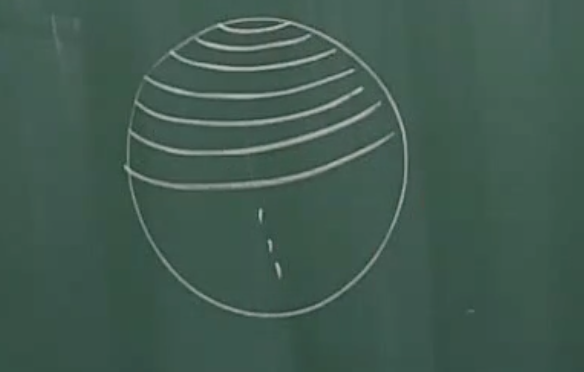
\includegraphics[width=0.5\textwidth]{images/lecture15_sphere1.png}

Далее покроем ее ''кирпичикам'' так, чтобы все стыки были т-образными:

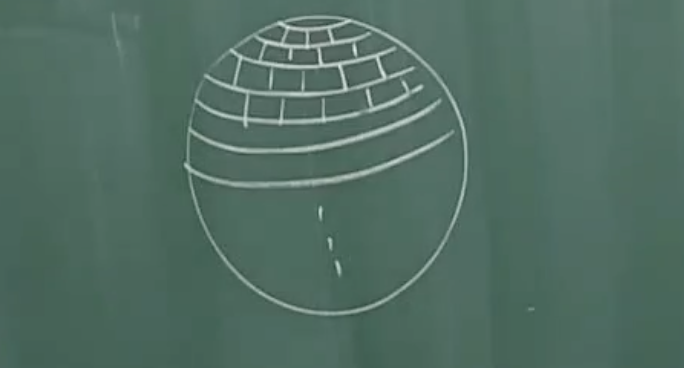
\includegraphics[width=0.5\textwidth]{images/lecture15_sphere2.png}

Рассмотрим объединение ''кирпичиков'', которые пересекаются с $A_1$ хотя бы по одной точке. Назовём это множество $G_1$.
Выберем кирпичики так, чтобы $diamG_1 < 1$. Через $\partial G$ обозначим его границу.\\
Утверждается, что $\partial G = L_1 \cup \dots \cup L_k$, где $L_i$ - замкнутые несамопересекающиеся ломаные, причем $L_i \cap L_j = \emptyset$.\\
Симметрично отразим $G_1$ относительно центра сферы. Назовём полученное множество $G_1'$. Заметим, что $G_1 \cap G_1' = \emptyset$, ведь $diamG <1$, то есть внутри $G$ нет противоположных точек. При этом $\partial G'$ симметрична $\partial G$ и $\partial G = L_1'+\dots+L_k'.$ Получили $2k$ замкнутых попарно непересекающихся ломаных на сфере. Из теоремы Жордана следует, что эти ломаные делят сферу на $2k+1$ связных частей. Их нечетно, значит, есть симметричная относительно центра сферы часть $B$, не лежащая при этом ни в $G_1$, ни в $G_1'$. Значит, $B$ покрывается $A_2 \cup A_3$. Таким образом у нас на сфере образовался связный ''пояс''. 

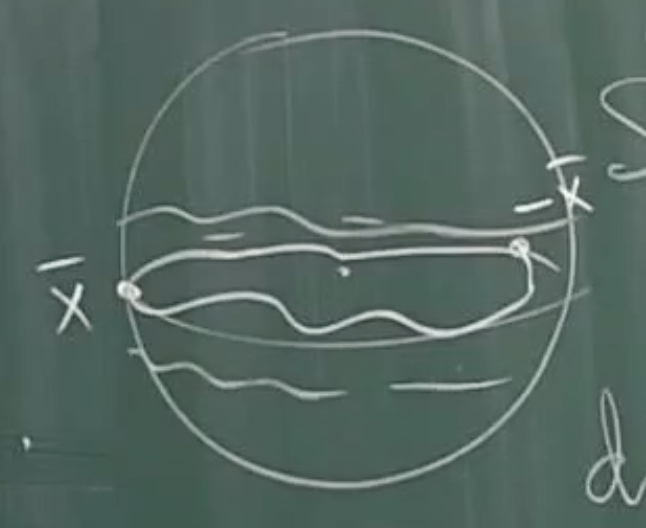
\includegraphics[width=0.5\textwidth]{images/lecture15_sphere4.png}

Возьмём в нём точку $\vv{x}$ и симметричную $\vv{-x} \in B$. Так как ''пояс'' связный, можем соединить эти две точки непрерывной кривой, не выходящей за его пределы.''Пояс'' центрально-симметричный, так что можно отразить её относительно центра. Но тогда, так как эта кривая покрывается $A_2 \cup A_3$ по теореме Борсука(теорема 1.24) для $\mathbb{R}^2$ найдутся две противположные точки, принадлежащие одному и тому же множеству.  

\end{proof}



\subsection{Хроматическое число $\mathbb{R}^n$}

\begin{theorem}(1972, Ларман, Роджерс)
\[
\chi(\mathbb{R}^n) \le (3+o(1))^n
\]

\end{theorem}

Если представить вершины графа $G(n,3,1)$ как векторы из нулей и единиц, то можно рассматривать его как дистанционный граф, в котором каждые две точки находятся на расстоянии $2$, ведь ребро проводится между ребрами, если скалярное произведение равно $1$. При этом мы знаем, что $\alpha(G(n,3,1)) \le n$.
Значит, \[
\chi(G(n,3,1)) \ge \frac{C_n^3}{n} \sim \frac{n^2}{6}.
\]
Аналогично можно рассмотреть граф $G(n,5,2)$. Мы знаем, что $\alpha(G(n,5,2)) \le C_n^2$(с помощью линейно-алгебраического метода). Тогда \[
\chi(\mathbb{R}^n) \ge \frac{C_n^5}{C_n^2} \sim \frac{n^3}{60}
\]

\begin{theorem}
Если $r - s = p^{\alpha}$, $p$ - простое, то \[\chi(\mathbb{R}^n) \ge \frac{C_n^r}{m(n,r,s)} \ge \frac{C_n^r}{\sum_{k = 0}^{r-s-1} C_n^k}\]

\end{theorem}